

%%%%%%% %%%%%%%%
\section{Summary statistics}

First, we fix some notation.
For a sample of individuals indexed by some set $A$,
genotyped at a set of genomic positions indexed by $S$,
the data are $\{G_{ijk} \; : \; i \in A, \; j \in S, \; k \in \{m,p\} \}$,
i.e.\ $G_{ijm}$ is the allele that the $i^\mathrm{th}$ individual inherited at the $j^\mathrm{th}$ position from her mother,
and $G_{ijp}$ is the corresponding allele inherited from her father.

Regardless of the process that has generated $G$, 
it makes sense to think about the sampling distribution of $G$,
and associated statistics --
i.e.\ the distribution of $G$ induced by some sort of random sampling of the individuals.
Often, we can actually obtain from $G$ a good estimate of the entire sampling distribution.
For instance, we can estimate the distribution of 
the the number of nucleotide differences between two individuals in a 100bp region
across all such regions and all pairs of sampled individuals,
as long as $G$ can be reasonably regarded as a random sample from some population.
We can further estimate conditional sampling distributions,
e.g.\ number of such differences as a function of geographical distance between them,
or in protein coding regions.

Here we relate the sampling distributions of a number of statistics easily computable form $G$
to sampling distributions of properties of the pedigree with recombination.

We will study aspects of the distributions of these statistics under various ``levels of sampling'':
\begin{enumerate}
  \item Unconditional, including averaging over the population process.
  \item Conditional on the population pedigree ($\pedigree$),
    and averaging over recombinations, segregation, and mutations.
  \item Conditional on the population ARG ($\meioses$), 
    averaging over choices of individuals.
  \item Conditional on the population ARG ($\meioses$),
    averaging over choices of locus.
\end{enumerate}
Only the first needs a population model.
The second is clearly fictitious, but can be useful (as we see below).
The latter two can be interpreted as empirical distributions.
Often, in practice, we have an empirical distribution obtained averaging across many loci (as in the last point),
and compare it to a theoretical distribution for a single locus under a population model.
This is in principle wrong, 
since it ignores correlations between loci introduced by the pedigree,
but in practice seems to be pretty good \citep{wakeley2012genealogies}.


%%%%%% %%%%%%% %%%%%%%%
\subsection{Number of segregating sites}

As a first example,
we can relate the mean and variance of the number of segregating sites in a sample
to the distribution of total time in the sample tree, simliar to the calculation of number of mutations in \citep{hudson1990gene}.
The number of segregating sites, $A_0$, in a sample of $k$ chromosomes at $|S|$ loci,
is the number of sites at which at least two of the sampled chromosomes differ.
For this to happen, there must have been a mutation at that site somewhere on the tree that relates the samples.

Concretely, suppose that we have sampled $k$ chromosomes,
and that (as above) the tree relating these samples at genomic position $x$ is $T_x$.
We measure ``length'' of the tree in meioses,
and denote by $|T_x|$ the total number of meioses the tree,
up until the most recent common ancestor.
Also, let $N_x$ denote the total number of mutations that have occurred at site $x$ during any of the meioses anywhere in $T_x$.
Under the usual assumption on mutations,
this number is Poisson distributed with mean $\mu |T_x|$.

Now let $X$ denote a randomly chosen locus,
$T = |T_X|$, and $N = N_X$.
It is straightforward that
\begin{align}
  \E[N] = \mu \E[T]
\end{align}
and using the formula for conditional partitioning of variance,
\begin{align}
  \var[N] &= \E[ \var[N|T] ] + \var[ \E[N|T] ] \\
    &= \E[ \mu T ] + \var[ \mu T ] .
\end{align}
Note that this remains true if $\mu$ depends on $x$.

Now, by linearity of expectation,
\begin{align}
  \E[A_0] = \E[ \sum_x N_x] = |S| \E[\mu T] .
\end{align}
Similarly, by conditioning on the collection of trees $\mathcal{T} = \{ T_x \st x \in S\}$,
since $N_x$ and $N_y$ are conditionally independent given $T_x$ and $T_y$,
\begin{align}
  \var[A_0] &= \E[ \var[A_0 | \mathcal{T} ] ] + \var\left[ \E[ A_0 | \mathcal{T} ] \right] \\
  &= \E \left[ \sum_{x,y\in S} \cov[N_x,N_y|\mathcal{T}] \right] + \var\left[ \sum_{x \in S} \E[ N_x | \mathcal{T} ] \right] \\
  &= \E \left[ \sum_{x\in S} \var[N_x|\mathcal{T}] \right] + \var\left[ \sum_{x \in S} \E[ N_x | \mathcal{T} ] \right] \\
  &= \E \left[ \sum_{x \in S} \mu |T_x| \right] + \var\left[ \sum_{x \in S} \mu |T_x| \right] \\
  &= \E \left[ \sum_{x \in S} \mu |T_x| \right] + \sum_{x,y \in S} \cov\left[ \mu |T_x|, \mu |T_y| \right] \\
  &= \mu |S| \E [ T ] + \mu^2 |S| \var[T] + \sum_{x \neq y \in S} \cov\left[ \mu |T_x|, \mu |T_y| \right] .
\end{align}
This agrees with \citet{hudson1990gene} if we are restricted to a single, nonrecombining locus.


%%%% %%%%%%% %%%%%%%
\subsection{Heterozygosity} 

The ``observed heterozygosity'' in a group of individuals in a genomic region 
is the probability that a randomly chosen individual is heterozygous at a randomly chosen nucleotide,
or 
\begin{align}
  H_O = \frac{ \# \left\{ (i,j) \st i \in A, \; j \in S, \; G_{ijp} \neq G_{ijm} \right\} }{ |S|\,|A| } ,
\end{align}
where $|S|$ denotes the total number of loci and $|A|$ denotes the total number of individuals.

In other words, $H_O$ is the proportion of homologous alleles that differ from each other, across $S$ and across $A$.
By calling them ``homologous'' we assume they share a common ancestor;
so if they differ there must have occurred a mutation since that common ancestor.
Take a single individual $i$,
suppose that the chance of a mutation occurring at site $j$ in a particular meiosis is $\mu_d$,
and that there have been $\tau_{ij}$ generations since the common ancestor of the maternal and paternal copies.
The probability that there has been no mutations since that time is $(1-\mu_d)^{2 \tau_{ij}}$,
since there are $2 \tau_{ij}$ meioses separating the two.
The proportion of heterozygous sites is determined by the empirical distribution 
of times back to the most common ancestor of paired homologous sites, averaged across sites and across individuals.
Let $\tau_H$ denote this distribution, i.e.\ $\P\{ \tau_H = t \} = \#\{ (i,j) \st \tau_{ij} = t \} / |S||A|$.
If, as assumed, there is no back mutation, then,
\begin{align}
  \E[ H_O \vert \meioses ] &= \frac{1}{|S|\,|A|} \sum_{i \in A} \sum_{j \in S} \left( 1 - (1-\mu_d)^{2 \tau_{ij}} \right) \\
      &= \E\left[ 1-(1-\mu_d)^{2 \tau_H} \right] \\
      &= \E\left[ 1-e^{-2 \mu \tau_H } \right] .
\end{align}
Note that $\tau_H$, if it was observable, would be a good \emph{summary statistic} (albeit complicated) of the pedigree,
and depends implicitly on the choice of individuals $A$ and the choice of genomic region $S$.
If $\mu$ is small, then $H_O \approx \mu \E[ \tau_H ]$,
i.e.\ the proportion of sites that an individual is heterozygous
is equal to the mutation rates multiplied by the average time back to the common ancestor of the maternal and paternal chomosomes.

Similarly, 
\begin{align}
  \var[ H_0 \vert \meioses ] &= \frac{1}{|S|\,|A|} \E\left[ e^{-2 \mu \tau_H } \left( 1 - e^{-2 \mu \tau_H } \right) \right] .
\end{align}
This implies that the observed heterozygosity $H_0$ is an estimtor of the statistic $\E[ \tau_H ]$ of the empirical distribution of pairwise coalescence times,
and that can put some explicit bounds on how good this estimator is.

As stated, $H_O$ is a single number, the chance that a randomly chosen homologous pair of alleles differ.
This averages over levels of relatedness of different individuals,
as well as mutation rates and depths of relatedness that may differ systematically across loci.
If we know local mutation rates, and partition sites according to this,
then we can estimate $H_O(\mu) = \E\left[ e^{-2 \mu \tau_H } \right]$ as a function of $\mu$,
obtaining an estimate of the Laplace transform of $\tau_H$.
% Comparing frequencies of heterozygosity in genomic windows of varying sizes 
% (i.e.\ using each 10bp window as one locus)
% has a similar effect,
% except that recombination makes this approximate.



\subsection{Mean number of pairwise differences}

Also known as ``expected heterozygosity'',
this is the chance that two randomly chosen alleles from $A$ at a random site in $S$ differ:
\begin{align}
  H_E &= \frac{ \#\{ (j,i_1,i_2,k_1,k_2) \st G_{i_1jk_1} \neq G_{i_2jk_2}  \} }{2|S|\,|A|(|A|-1)}  .
\end{align}
$H_E$, like $H_O$, is computable from the distribution of the number of generations available for mutation 
where the relevant number of generations here is defined to be $\tau_T$.
Concretely, $\tau_T$ is the number of generations back to the common ancestor
at a uniformly chosen locus
between two uniformly chosen chromosomes in the population
(possibly, but not necessarily, in the same individual).
Again,
\begin{align}
  H_E &= \E\left[ (1-\mu_d)^{2 \tau_T} \right] = \E\left[ e^{-2 \mu \tau_T} \right] .
\end{align}


Such measures of heterozygosity can measure not only within-group diversity
but also between-group divergence,
by computing e.g.\ the probability that two randomly chosen individuals
in different subpopulations
differ at a randomly chosen locus.
Any such measurement can be thought of as the proportion
of some subset of paths through the pedigree
along which a mutation has occurred;
(crucially) assuming that the mutation process is independent of inheritance,
this probability of mutation only depends on the number of meioses along the path,
and hence on the distribution of path lengths.
Above these distributions of lengths across certain sets of paths through the pedigree
appeared as $\tau_H$ and $\tau_T$.



%%%%%%% %%%%%%%%
\subsection{The allele frequency spectra}

Mutations at a locus induce a partition of a set of chromosomes --
those who are identical at that locus.
Heterozygosities are pairwise statistics;
when comparing two chromosomes there are only two possible results:
identical or not.
When looking at larger samples, any partition is possible;
at loci with no more than two alleles, all dichotomous partitions are possible.

\begin{figure}[ht!]
  \begin{center}
    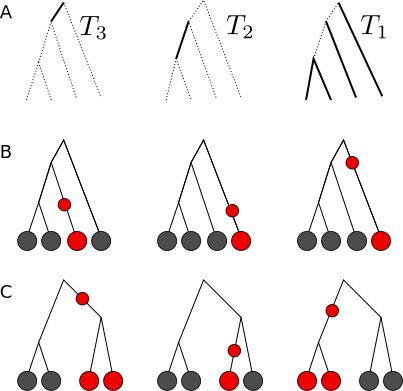
\includegraphics[width=3.5in]{frequency-spectra-trees}
  \end{center}
  \caption{
  \textbf{(A)} The lengths $T_3$, $T_2$, and $T_1$ (see text).
  Note that mutations on $T_3$ are indistinguishable from those on  $T_1$ if the alleles are not polarized.
  \textbf{(B--C)}
  The frequency spectrum encodes information about distributions of tree shape:
  the lower set of trees has longer internal branches, and so will have a higher chance of 2:2 partitions
  than the upper set of trees.
  Mutations (circles on the tree) separate ``red'' from ``black'' types;
  assuming that mutation is independent of the pedigree implies
  that the location of mutation is uniform (proportional to length) on the tree.
  \label{fig:frequency_spectra_trees}
  }
\end{figure}

Suppose we are looking at the empirical distribution of allele frequencies in a sample of size $|A|=n$
at biallelic sites, including only the polymorphic sites, i.e.\ the sites where more than one allele is seen in the sample.
This is called the ``allele frequency spectrum'', or ``site frequency spectrum''.
Let $(N_{j,0},N_{j,1})$ denote the numbers of sampled chromosomes that have the `0' and `1' alleles, respectively,
and define $F_k$ to be the number of sites with the allele `1' is at frequency $k$, or
\begin{align}
  F_k &= \frac{ \#\{ j : N_{j,0} = k \} }{ |S| } \quad & k &\in \{0,1,\ldots,n\} \\
\end{align}
and the ``unfolded'' and ``folded'' allele frequency spectra 
\begin{align}
  a_k^* &= \frac{ F_k }{ F_1 + \cdots + F_{n-1} }
  a_k &= \begin{cases} 
    \frac{ F_{n/2} }{ F_1 + \cdots + F_{n-1} } \qquad \text{if } k = n/2 \\
    \frac{ F_k + F_{n-k} }{ F_1 + \cdots + F_{n-1} } \qquad \text{if } k \neq n/2 
  \end{cases} \\
\end{align}
If we have some way of polarizing mutations, so that e.g.\ allele `0' is more likely to be the ancestral allele,
then the unfolded spectrum is more useful;
otherwise, if the choice of allele labeling is arbitrary, 
we expect $a_k^* = a_{n-k}^*$ and the folded spectrum is more natural.

Now, we'll compute the mean and variance of $F_k$
conditional on the ARG $\meioses$, averaging across the mutation process.
Let $\tree_j$ be the gene three at site $j$,
and let $T_{j,k}$ be the total length of branches in $\tree_j$ subtended by exactly $k$ tips,
so that $|\tree_j| = \sum_{k=1}^{n-1} T_{j,k}$
(see figure \ref{fig:frequency_spectra_trees}).
Again assuming that the mutation is independent of inheritance,
the probability that site $j$ has no segregating mutation is $\exp(-\mu |\tree_j|)$,
and the probability that only a single segregating mutation has occurred is $\exp(-\mu |\tree_j|) \mu |\tree_j|$.
Given that only a single mutation has occurred,
the location of that mutation is uniform on the tree,
and so the probability that a mutation occurs at frequency $k$ at site $j$ is
\[
\P\{ N_{j,1}=k \vert \tree_j \}
  % = \frac{ T_{j,k} }{ |\tree_j| }  \mu |\tree_j| \exp(-\mu |\tree_j|) 
  = \mu T_{j,k}  \exp(-\mu |\tree_j|)  = \mu T_{j,k} + O(\mu^2 |\tree_j|^2).
\]
Therefore, 
\begin{align}
  \E[ F_k \vert \meioses ] &= \sum_j \P\{ N_{j,1}=k \vert \tree_j \} \\
        &= \mu \sum_j T_{j,k}  \exp(-\mu |\tree_j|) ,
\end{align}
and
\begin{align}
  \var[ F_k \vert \meioses ] &= \mu \sum_j T_{j,k}  \exp(-\mu |\tree_j|) \left( 1 - \mu T_{j,k}  \exp(-\mu |\tree_j|) \right).
\end{align}

Therefore, 
\begin{align}
  \E[ a^*_k \vert \meioses ] &= XXX
\end{align}

the expected contribution of sites with only a single segregating mutation
to $a_k^*$ is $\E\left[ \exp(-\mu |T|) \mu T_k \right]$.
to first order in $\mu |T|$, this says that $a_k^*$ is $\E[T_k]/\E[|T|]$,
the average total number of ancestors of exactly $k$ of the samples
divided by the average total number of ancestors up until the most recent common ancestor of all $n$ samples.


This distribution is obtained by averaging across loci.
Pick a random locus, and call the tree relating the samples at that locus $T$.
Let $|T|$ denote the total length of the tree (in meioses),
and $T_k$ denote the total length of all branches in the tree that are subtended by exactly $k$ tips,
for $1 \le k \le n-1$, so that $|T| = \sum_{k=1}^{n-1} T_k$.



%%%%%%% %%%%%%%%
\subsection{Linkage}

The previous statistics were \emph{single-site} statistics
that took their information from the branching structure of the pedigree
and the differentiating action of mutation along it.
Consideration of the relationships multiple loci brings recombination into the picture.
Perhaps the simplest summary of this is the measure of \emph{linkage disequilibrium}.
It is a two-site statistic, and is in some sense is a single-individual statistic.

Take two sites $\ell_1$ and $\ell_2$, at recombination distance $r$,
so that mean number of crossovers that fall between them in a generation is $r$.
One statistic measuring association between alleles $A_1$ and $A_2$ at $\ell_1$ and $\ell_2$ is
\begin{align}
  D_{\ell_1 \ell_2}(A_1,A_2) = P_{\ell_1 \ell_2}(A_1 A_2) - P_{\ell_1}(A_1) P_{\ell_2}(A_2) ,
\end{align}
where $P_{\ell_1 \ell_2}(11)$ is the empirical frequency of chromosomes that have the `1' allele at both sites $\ell_1$ and $\ell_2$,
and $P_{\ell_1}(1)$ is similar.
To measure association between the loci we sum over alleles and square, defining
\begin{align}
  D_{\ell_1 \ell_2}^2 &= \left( \sum_{A_1,A_2} D_{\ell_1 \ell_2}(A_1,A_2) \right)^2 \\
    &= \sum_{A_1,A_2} \left( P_{\ell_1 \ell_2}(A_1 A_2) - P_{\ell_1}(A_1) P_{\ell_2}(A_2) \right)^2
\end{align}

% Also,
% \[
% D_{\ell_1 \ell_2} = \cov[ \one_{X_1=A_1}, \one_{X_2=A_2} ]  .
% \]

Now assume that the loci are biallelic, coded as $\{0,1\}$
(in which case $D_{\ell_1 \ell_2}^2  = 4 \left( P_{\ell_1 \ell_2}(1 1) - P_{\ell_1}(1) P_{\ell_2}(1) \right)^2$)
and let $I$, $J$, $K$, and $L$ be the indices of individuals chosen uniformly at random with replacement.
Now let $X_I$ be a randomly chosen allele at locus $\ell_1$ for $I$ (i.e.\ either $G_{I\ell_1m}$ or $G_{I\ell_1p}$),
$Y_I$ be the same for locus $\ell_2$, on the same chromosome as $X_I$,
and similarly for $J$, $K$, and $L$.
Then
\begin{align}
  D_{\ell_1 \ell_2}^2 = \P\{ X_I = X_J \& Y_I = Y_J \} - 2 \P\{ X_I = X_J \& Y_I = Y_K \} + \P\{ X_I = X_J \& Y_K = Y_L \} .
\end{align}
(Note: this is an example of the more general idea of a ``distance covariance'', here between $X_I$ and $Y_I$.)

These quantities are things that we can compute in terms of paths through the pedigree
if we can assume that the appearance of mutations can be taken as independent of the pedigree.
Let $\tau_1(I,J)$ be the number of generations back to the common ancestor of the chosen chromosomes of $I$ and $J$ at locus $\ell_1$,
and similarly for $\tau_2(I,J)$ at locus $\ell_2$.
Then under the infinite alleles model,
with mutation rate $\mu$, 
\begin{align}
  \P\{ X_I = X_J \& Y_K = Y_L \} &= \E[ \exp(-2\mu(\tau_1(I,J)+\tau_2(K,L))) ] .
\end{align}
Similar equations for the other terms leads to
\begin{align}
  D_{\ell_1 \ell_2}^2 &= \E[ \exp(-\mu(\tau_1(I,J)+\tau_2(I,J))) ] - 2 \E[ \exp(-2\mu(\tau_1(I,J)+\tau_2(I,K))) ] + \E[ \exp(-2\mu(\tau_1(I,J)+\tau_2(K,L))) ] \\
    &= \cov[ e^{-2\mu\tau_1(I,J)}, e^{-2\mu \tau_2(I,J)} ] - 2 \cov[ e^{-2\mu\tau_1(I,J)}, e^{-2\mu \tau_2(I,K)} ] + \cov[ e^{-2\mu\tau_1(I,J)}, e^{-2\mu \tau_2(K,L)} ] \\
    &\approx 2\mu^2 \left( \cov[ \tau_1(I,J),  \tau_2(I,J) ] - 2 \cov[ \tau_1(I,J),  \tau_2(I,K) ] + \cov[ \tau_1(I,J),  \tau_2(K,L) ] \right) ,
\end{align}
where the latter approximation holds if the expected number of mutations per site ($\mu \tau$) is small.


What does $D_{\ell_1 \ell_2}^2$ have to say about the structure of the ancestral recombination graph?
Intuitively, since it is the squared correlation between alleles at two loci on the same chromosome,
it should be telling us about how much those loci tend to stick together.
This is reflected in the formula above, which interprets $D_{\ell_1 \ell_2}^2$
in terms of covariances of times back to most recent common ancestors at the two sites.

We can do a little more to make these covariances interpretable,
in terms of the recombination distance between $\ell_1$ and $\ell_2$.
For convenience, let $Z_1(I,J) = e^{-2\mu \tau_1(I,J)} - \E[e^{-2\mu \tau_1(I,J)}]$, etcetera.
Again assuming independence of mutation and the pedigree,
given $\tau_1(I,J)$,
the probability that there was no recombination between the loci along the path between $I$ and $J$
is $\exp(- 2r\tau_1(I,J))$;
in this case, $\tau_1(I,J) = \tau_2(I,J)$.
Suppose that in the complimentary case, when there was recombination, that $\tau_2$ is (conditionally) independent of $\tau_1$ --
not true, but not too bad either.
The correponding term in the formula for $D_{\ell_1 \ell_2}^2$ decays exponentially with $r$:
\begin{align}
  \cov[ e^{-2\mu\tau_1(I,J)}, e^{-2\mu \tau_2(I,J)} ] &= \E[ Z_1(I,J) Z_2(I,J) ]  \\
        &\approx \E\left[ e^{-2r \tau_1(I,J)} Z_1(I,J)^2  \right] \\
        &= \E\left[ e^{-2r \tau_1(I,J)} \left( e^{-2\mu \tau_1(I,J)} - \E[e^{-2\mu \tau_1(I,J)}] \right)^2 \right] .
\end{align}

Now take the second term.
The most obvious way that the genealogy induces correlations between $\tau_1(I,J)$ and $\tau_2(I,K)$
occurs if the most recent common ancestor of $I$ and $J$ is the same as that of $I$ and $K$,
in which case $\tau_1(I,J) = \tau_1(I,K)$ (see figure \ref{fig:coal_time_correlation}A),
and there is no recombination along the whole genealogy back to this MRCA.
Define $\tau_1(I,J,K)$ to be the age of this MRCA.
If we now assume that the case in which there was a recombination on the path from $I$ to $K$ contributes nothing to the covariance,
since the probability that $I$ is in this position is $1/3$,
\begin{align}
  \E[ \exp(-2\mu(\tau_1(I,J)+\tau_2(I,K))) ] &= \E[ Z_1(I,J) Z_2(I,K) ] \\
  &\approx \E \left[ e^{-2r \tau_1(I,J,K)} Z_1(I,J)^2 \vert \tau_1(I,J) = \tau_1(I,J,K)  \right] \\
  &= \frac{1}{3} \E \left[ e^{-2r \tau_1(I,J,K)} \left( e^{-2\mu \tau_1(I,J,K)} - \E[e^{-2\mu \tau_1(I,J)}] \right)^2 \right] .
\end{align}


\begin{figure}[ht!]
  \begin{center}
    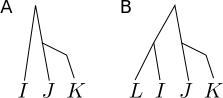
\includegraphics{coal-time-correlation}
  \end{center}
  \caption{
    \textbf{(A)} The tree topology in which the most recent common ancestor of $I$ and $J$ 
    is the same as the most recent common ancestor of $I$ and $K$, so that $\tau(I,J) = \tau(I,K)$.
    \textbf{(B)} Similar, but $\tau_{I,J} = \tau_{K,L}$ -- note that exchanging $K$ and $L$ would work as well.
    \label{fig:coal_time_correlation}
  }
\end{figure}

It should be clear what to do for the third term now.
If the situation in figure \ref{fig:coal_time_correlation}B occurs (which it does with probability $1/6$)
then $\tau_1(I,J) = \tau_1(K,L)$.
As before,
\begin{align}
  \E[ \exp(-2\mu(\tau_1(I,J)+\tau_2(K,L))) ] &= \E[ Z_1(I,J) Z_2(K,L) ] \\
  &\approx \E \left[ e^{-2r \tau_1(I,J,K,L)} Z_1(I,J)^2 \vert \tau_1(I,J) = \tau_1(I,J,K,L)  \right] \\
  &= \frac{1}{6} \E \left[ e^{-2r \tau_1(I,J,K,L)} \left( e^{-2\mu \tau_1(I,J,K,L)} - \E[e^{-2\mu \tau_1(I,J)}] \right)^2 \right] .
\end{align}

Combining these gets us an approximate expression for $\E[D_{j_1 j_2}^2]$ 
that is a tad unwieldy,
but is in terms of ages of most recent common ancestors of two, three, and four samples:
taking only terms first-order in $\mu$,
and letting $t = \E[\tau_1(I,J)]$,
\begin{align}
  \E[ D_{j_1 j_2}^2 ] &\approx 4 \mu^2 \E\left[
    e^{-2r \tau_1(I,J)} ( \tau_1(I,J) - t )^2 
    - \frac{2}{3} e^{-2r \tau_1(I,J,K)} ( \tau_1(I,J,K) - t )^2 
    + \frac{1}{6} e^{-2r \tau_1(I,J,K,L)} ( \tau_1(I,J,K,L) - t )^2 
    \right] .
\end{align}


